\chapter{Estado del Arte\label{sec:estado_del_arte}}

Hoy en día, resulta complicado imaginar Internet como una red exclusiva de clientes y servidores. El fenómeno ``Internet of Things''~\cite{Atzori20102787} ha supuesto un cambio radical a hora de percibir que es Internet. Del mismo modo, que resulta difícil imaginarse a alguien sin un smartphone~\cite{bib:introduccion:smartphone} o sin acceso a Internet~\cite{bib:internet:growth}. Este crecimiento ha supuesto un equivalente aumento tanto en la velocidad como en tamaño de las redes internas de las empresas.

Para mantener una red de cierto tamaño en un buen estado, es necesario monitorizarla~\cite{de2013proactive}. Comunmente se habla de 2 tipos de monitorización: Activa y Pasiva. Cada tipo de monitorización ofrece una serie de ventajas e inconventientes. La \gls{mactiva}, permite a un administrador de red conocer el estado y la calidad de una red, pues este tipo de mediciones ofrece métricas como ancho de banda disponible, el jitter de la red (El cual es muy importante a la hora de transmitir contenido multimedia~\cite{dpdk:Leir1306,hernandomeasuring,garcia2014low}) o la latencia de la red entre dos extremos. No obstante, la monitorización activa afecta de mayor o menor forma al estado de una red, lo que puede perjudicar a la medida y por supuesto a los usuarios de la propia red. Estos efectos perjudiciales, pueden verse ampliados si la monitorización no se realiza mediante técnicas adecuadas~\cite{Ramos20111435}.

Por otro lado, la \gls{mpasiva} no sufre de los efectos perjudiciales de la \gls{mactiva}. Aunque este tipo de monitorización no es capaz de medir el jitter entre dos puntos de la red, ni tampoco la latencia a la que se ven sometidas determinadas comunicaciones, si ofrece otras muchas métricas relevantes. Para realizar este tipo de monitorización en una enlace de alta velocidad, es necesario un equipo de elevadas prestaciones para capturar el tráfico~\cite{dpdk:netfpga,dpdk:packetshader,moreno2012TFM,dpdk:victor:ref:1,dpdk:victor:ref:2,dpdk2015}.

Al disponer de todo el tráfico de un enlace, es posible obtener métricas de este, como pueden ser el ancho de banda del propio enlace, o de una determinada aplicación o usuario, la detección de intrusiones o incluso detección de malfuncionamiento de determinadas aplicaciones.
Aunque las posibilidades de la \gls{mpasiva} son muchas, tratar con toda esta cantidad de tráfico también supone una gran carga computacional. Por ello, existe multitud de investigación acerca de como escoger el tráfico que debe ser posteriormente almacenado o procesado.
Una de las aproximaciones más conocidas para segmentar el tráfico, es lo que se llama \textit{packet sampling}~\cite{1209210}. Este tipo de algoritmos intentan seleccionar el tráfico más relevante, de forma que sea posible obtener información estadística de ellos y a su vez reducir de manera drástica el número de paquetes por segundo que deben ser procesados. No obstante, utilizar \textit{packet sampling} tiene un cierto impacto en la medida~\cite{Brauckhoff:2006:IPS:1177080.1177101}, además de limitar el número de métricas interesantes que pueden obtenerse a partir de la \gls{mpasiva}.

Otros métodos de selección de tráfico, se basan en la selección por protocolo. Dado que existen miles de protocolos, es posible que de cara a realizar una monitorización solo nos preocupen algunos en concreto. Aunque identificar un protocolo a nivel de red o transporte es una tarea trivial, no lo es a la hora de identificar un protocolo a nivel de aplicación~\cite{dpdk:Leir1306}. Por este motivo, existen 3 formas diferentes de clasificar tráfico: por puerto, mediante clasificación estadística o mediante \gls{dpi}.
La clásica clasificación por puerto, nos brinda velocidad en la clasificación, pero no es útil al a hora de clasificar protocolos sin puertos conocidos, detectar atacantes o errores de configuración. La clasificación estadística por otro lado, nos brinda un compromiso entre fiabilidad y velocidad, lo que ha propiciado una elevada cantidad de investigación~\cite{dpi:critica:3,dpi:critica:7,dpi:critica:8,dpi:critica:13}. No obstante, la clasificación estadística requiere disponer de una muestra preliminar del tráfico a partir de la cual obtener un modelo que utilizar posteriormente. De igual modo, es complicado confiar en este tipo de métricas si se desea aplicar algún tipo de reacción activa como denegar a un usuario el acceso a un recurso, a pesar de que la métrica acierte en el 99\% de los casos.
En el caso de \gls{dpi}, es necesario aplicar una gran cantidad de cálculo para obtener el resultado~\cite{dpi:critica:10b}. Por ello, se han desarrollado aplicaciones de \gls{dpi} que recurren a diversos coprocesadores como \glspl{gpu}~\cite{dpi:gnort,dpdk:Leir1306} o \glspl{fpga}~\cite{dpi:tfm:6,dpi:tfm:7,dpi:tfm:8,dpi:tfm:11}.
La propia detección de protocolos, aporta suficiente información como para la construcción de firewalls~\cite{dpi:juancho:master,dpi:pedro:2}, detección de intrusiones~\cite{dpi:gnort}, corrección de \gls{qos}~\cite{dpdk:Leir1306} entre otras muchas aplicaciones.

En redes de altas velocidades, en muchos casos resulta poco verosímil trabajar a nivel de paquete y frecuentemente resulta poco interesante. Por este motivo, la extracción de la información de flujo con su correspondiente análisis se vuelve fundamental~\cite{fp:pedroth}. Aunque generar la información de cada uno de los flujos supone procesar igualmente cada uno de los paquetes, resulta un proceso computacionalmente más barato que una clasificación \gls{dpi}. Este procesado de flujos tiene una gran cantidad de desarrollo por detrás ya que facilita el análisis posterior de una red. El tratamiento de flujos es un tema extenso, desde los estándar de NetFlow~\cite{claise2004cisco,rt:netflow} e IPFIX~\cite{hofstede14surveys,claise2008specification}, hasta el desarrollo de herramientas para \gls{cpu}~\cite{mckeown2008openflow,kimCOMCOM06,garcia2014low,fp:pedroth} o para diversos coprocesadores~\cite{fp:marco}.

En definitiva, para poder analizar la información de los flujos de una red, obtener la información referente a los protocolos o simplemente transmitir y recibir paquetes a alta velocidad, es necesario un conjunto de herramientas capaz de capturar y emitir el tráfico exprimiendo todo el ancho de banda del enlace.

\newpage
\lsection{Herramientas de captura}

Realizar un proceso de captura a alta velocidad en un ordanador convencional, supone atravesar toda la pila de red de un sistema operativo, lo que de forma inevitable nos supone una degradación del rendimiento y en el caso de redes de $\geq$10~Gbps, un impedimento a la hora de capturar todo el tráfico. Para solventar este problema, se han desarrollado multitud de herramientas y hardware dedicado. Dos claros ejemplos de hardware dedicado son los procesadores de red Tilera~\cite{bib:tilera} y las FPGAs, en especial con su popular proyecto NetFPGA~\cite{dpdk:netfpga}.
No obstante, trabajar con este tipo de harware supone un alto coste de programación, pues los sistema tienen una complejidad elevada. Por el otro lado, estos sistemas permiten realizar algunas tareas que en software serían mucho más complejas o incluso inviables. Algunos de los trabajos más interesantes en estas plataformas son: Procesamiento \gls{dpi} a 200~Gbps sobre una Tilera~\cite{bib:tilera:dpi200}, captura y almacenamiento a disco a 10~Gbps~\cite{zazo2014tnt10g}, emisión de tráfico a 10~Gbps con precisión de ns~\cite{zazo2014tnt10g}, obtención de estadística de flujos~\cite{fp:marco} o marcado temporal de paquetes con precisión GPS~\cite{garnica2010argos,kaemmerer2015method}.

 No obstante, para la mayoría de aplicaciones de red, no es necesario recurrir al hardware dedicado. Por ello, se han desarrollado multitud de herramientas que intentan exprimir al máximo el hardware disponible. Aunque cada una de las aplicaciones toma una serie de decisiones diferentes, en su conjunto todas intentan reducir el impacto de la pila de red, así como el número de interrupciones del procesador. A continuación se muestran algunas de las herramientas más populares y potentes en captura y procesado de red, así como su funcionamiento y características.
 
\subsection{PF\_RING DNA}
\textit{PF\_Ring}~\cite{RizzoDMA,libzeroNTOP} es un motor y un framework de captura para las tarjetas Intel de 1 y 10~Gbps. Este motor, está diseñado para explotar sistemas \gls{multicore}, de forma que el tráfico de una única \gls{nic}, se divida de forma equitativa entre diferentes colas de paquetes. Cada una de estas colas, debe ser gestionada por un único \gls{core}. De esta forma, cada \gls{core}, es el encargado de solicitar las copias de la memoria de la tarjeta hasta la memoria principal, así como de atender a las interrupciones de la tarjeta de red asociadas a la cola que está atendiendo.
De esta forma, el motor permite paralelizar el proceso de captura adquiriendo un enorme speedup. No obstante, hay que tener en cuenta la arquitectura de la máquina subyacente, pues una tarjeta de red está conectada a un único procesador. Dado que nos encontramos en una arquitectura de \gls{numa}, instanciar más colas que \glspl{core} tiene el procesador, supondrá que el otro procesador se verá obligado a procesar también tráfico. Esto causará que el segundo procesador interrumpirá al primero para poder acceder a la tarjeta, pudiendo perjudicar el rendimiento.

Otro detalle de la implementación de \textit{PF\_Ring}, se encuentra en las copias de paquetes. Realizar una copia en memoria tiene un coste que se vuelve no despreciable a la hora de hablar de 10~Gbps. Por este motivo, \textit{PF\_Ring} sigue la política de \gls{zerocopy}, de forma que una vez llegan los paquetes a la tarjeta, \textit{PF\_Ring} copia el contenido de los paquetes a la memoria principal y mapea dicha memoria al usuario. De esta forma, queda evitada la copia entre la zona de memoria del usuario y el espacio del módulo del kernel.
Es importante destacar que \textit{PF\_Ring} proporciona una API en formato estándar de facto: \textit{libPCAP}.
En la figura~\ref{fig:flow:pfring} se muestra el flujo de datos que siguen los paquetes hasta llegar a una aplicación de usuario.

\begin{figure}[!bth]
\centering
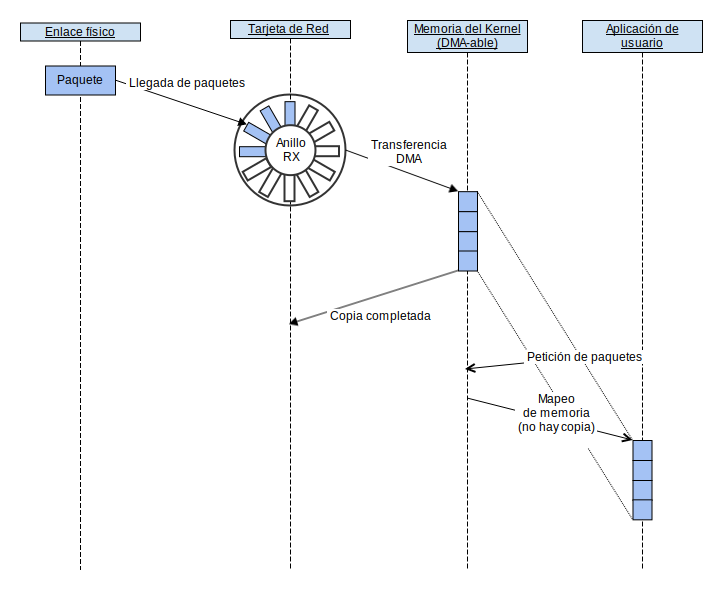
\includegraphics[scale=.6]{pfring}
\caption{Flujo de paquetes en PF\_Ring}
\label{fig:flow:pfring}
\end{figure}

\newpage
\subsection{PacketShader}
A pesar de que \textit{PacketShader}~\cite{dpdk:packetshader} fue diseñado inicialmente para ser un router, con la ayuda de una \gls{gpu}, el núcleo de este sistema puede ser extrapolado a otras aplicaciones.
Este motor, cuenta con capacidad de trabajar a tasas de varias decenas de~Gbps, ya que al igual que \textit{PF\_Ring}, explota los beneficios del paralelismo, así como una reducción en el número de copias. No obstante, cabe destacar en que este sistema utiliza el método de \gls{onecopy} en vez de \gls{zerocopy}, lo que puede llegar a degradar el rendimiento del motor de captura. 

Algunas de las optimizaciones de \textit{PacketShader} es el control de \gls{cache}. Toda la memoria se encuentra alineada de forma que las \glspl{cache} de la \gls{cpu} sufran lo menos posible, optimizándose así el rendimiento.
Como desventaja, cabe indicar que el motor no pide datos nuevos a la tarjeta hasta que el usuario no lo solicita, pudiéndose así perder paquetes si el usuario no hace las llamadas en el tiempo adecuado. A diferencia con \textit{PF\_Ring}, \textit{PacketShader} no provee una API de uso estándar, por lo que un posible desarrollador usuario se vería obligado a reescribir parte de su aplicación de red. 
En la figura~\ref{fig:flow:ps} se muestra el flujo de datos que siguen los paquetes hasta llegar a una aplicación de usuario.


\begin{figure}[!bth]
\centering
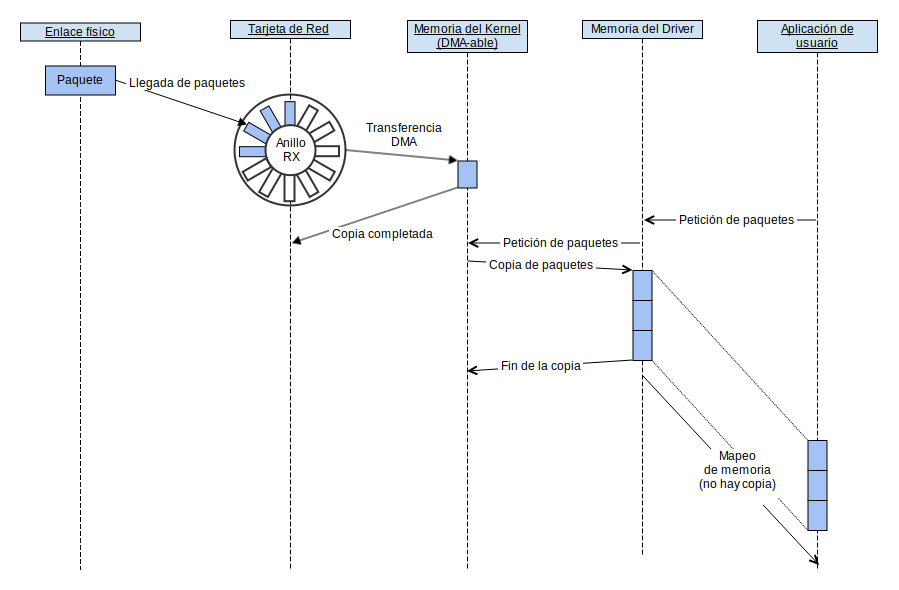
\includegraphics[scale=.6]{ps}
\caption{Flujo de paquetes en PacketShader}
\label{fig:flow:ps}
\end{figure}

\newpage
\subsection{HPCAP}
El driver \textit{HPCAP} fue desarrollado en el grupo de investigación HPCN~\cite{moreno2012TFM}. Este driver, es una extensión mejorada del driver oficial de las tarjetas Intel de 10~Gbps, por lo que solo es compatible con este tipo de tarjetas. Al ser una extensión, este motor de captura conserva en gran medida parte de la funcionalidad original del driver, permitiendo a las interfaces funcionar un modo \gls{vanilla} o en modo \textit{HPCAP} indistintamente. Al contrario que los otros motores de captura presentados anteriormente, \textit{HPCAP} tiene la capacidad de capturar la mayor parte del tráfico con una única cola de recepción.

Al igual que \textit{PacketShader}, \textit{HPCAP} se basa en la filosofía de \gls{onecopy}. Aunque a primera vista está claro que la filosofía del \gls{zerocopy} proporciona una copia menos y mejora el rendimiento, esta técnica supone mantener en memoria los paquetes hasta que el último de los procesos haya terminado con él. Dado que la zona de memoria en la que puede escribir la tarjeta es pequeña, si el tiempo total de proceso de un paquete es elevado, la tarjeta se quedará sin espacio donde copiar los nuevos paquetes viéndose obligada a descartar algunos de ellos. En el caso de la filosofía \gls{onecopy}, es posible mantener un buffer intermedio de gran tamaño en donde almacenar temporalmente los paquetes recibidos. De esta forma, es posible a su vez crear pipelines de proceso de paquetes mucho mayores y mantener un cierto aislamiento de las aplicaciones de procesado de red y la captura en sí, elemento del que no dispone la implementación de \textit{PacketShader}.
Como cierta desventaja, desear utilizar el motor de captura \textit{HPCAP} en modo \textit{HPCAP}, requiere utilizar una API proporcionada por el propio motor obligando a un desarrollador a reescribir su programa de procesado de red.
En la figura~\ref{fig:flow:hpcap} se muestra el flujo de datos que siguen los paquetes hasta llegar a una aplicación de usuario.


\begin{figure}[!bth]
\centering
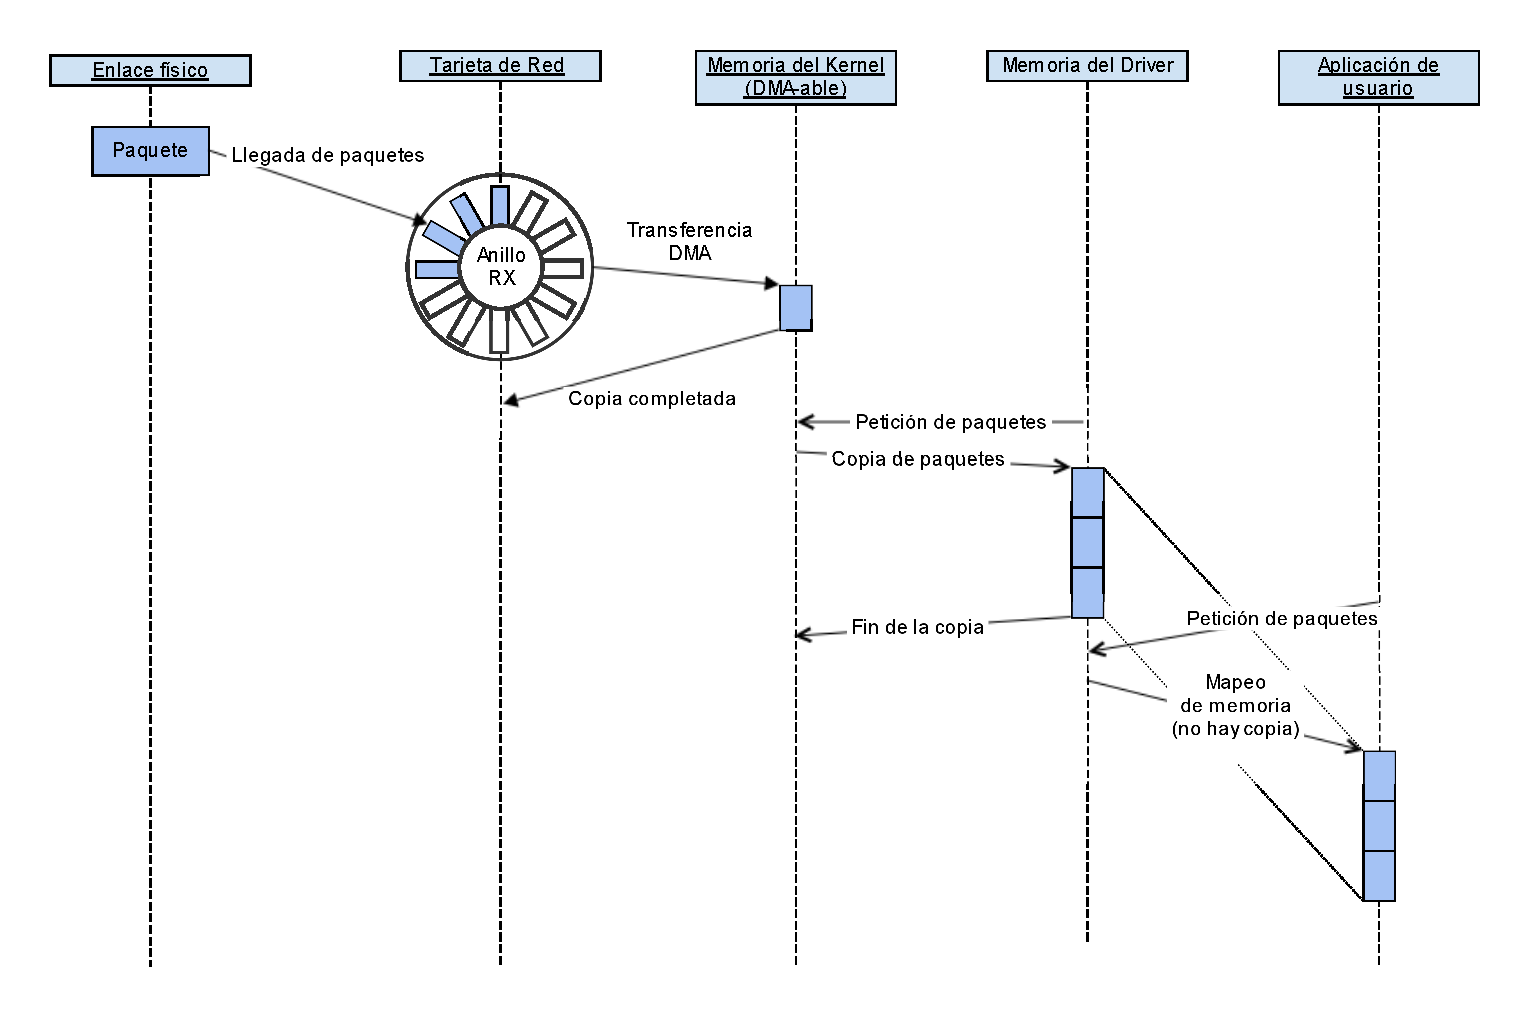
\includegraphics[scale=.6]{hpcap}
\caption{Flujo de paquetes en Hpcap}
\label{fig:flow:hpcap}
\end{figure}

\newpage
\subsection{Intel DPDK}
Intel \gls{dpdk}, es una filosofía, así como un motor de captura~\cite{dpdk:whitepaper:whydpdk,dpdk2015}. Se trata de uno de los sistemas de captura mas novedosos, y por ello, cuenta con gran cantidad de las filosofías que se han ido desarrollando previamente. La filosofía de Intel \gls{dpdk}, se basa en explotar la tecnología multicore de los sistemas actuales, de forma que uno o varios hilos, sean los encargados de recibir y transmitir los datos por una determinada \gls{nic}. En paralelo, otros hilos serán los encargados de procesar dicho tráfico (por ejemplo enrutar, o realizar \gls{dpi}), y si es oportuno, enviar de nuevo los paquetes a los hilos que manejan las transmisiones. Todo esto, de una manera relativamente transparente mediante la utilización de anillos (Colas circulares) para conectar los diferentes hilos entre sí. Un ejemplo de este tipo de arquitectura puede verse en la figura~\ref{fig:flow:dpdk}. 

A pesar de ser un motor de captura (y transmisión) desarrollado por Intel, \gls{dpdk} da soporte a multitud de tarjetas de red no fabricadas por la propia compañía. Algunas de las tarjetas soportadas es la ellas, son las tarjetas Ethernet a 40~Gbps Mellanox o las tarjetas \textit{enic} de \textit{Cisco}. Del mismo modo que \gls{dpdk} da soporte a diversas tarjetas, tambien da soporte a elementos virtualizados como a las propias \glspl{nfv} de sus \glspl{nic}, o las tarjetas paravirtualizadas con \gls{virtio}.
Intel \gls{dpdk} evita utilizar el espacio del Kernel de linux para maniobrar (evitando así copias intermedias). Por este motivo, su diseño se basa en la construcción de pequeños drivers a nivel de usuario (mediante el módulo \textit{UIO} de \textit{Linux}), lo que permite a un desarrollador utilizar la API de \gls{dpdk} sin tener que preocuparse por los problemas de trabajar a nivel de Kernel.
Esto mismo, llevó a \gls{dpdk} a optar por la filosofía de \gls{zerocopy}, la cual, puede llegar a ser perjudicial si el pipeline de proceso se llegase a alargar demasiado.


\begin{figure}[!bth]
\centering
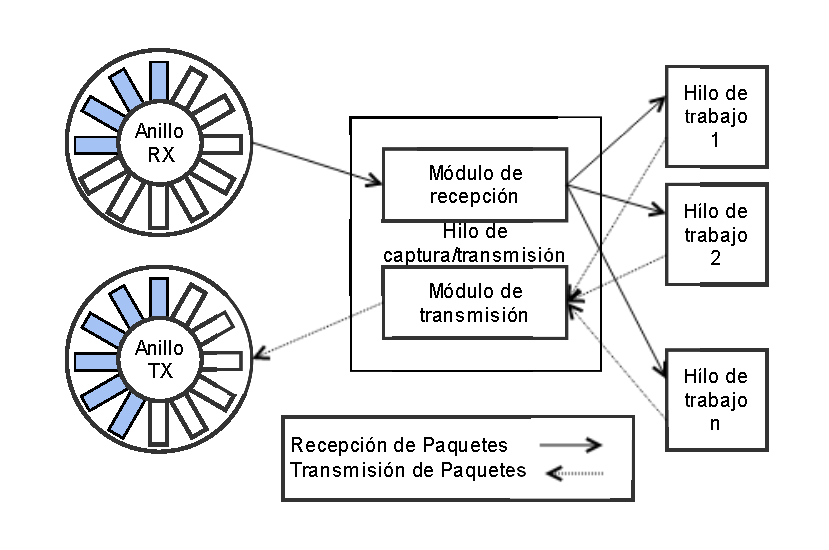
\includegraphics[scale=.6]{dpdk}
\caption{Flujo de paquetes en una aplicación Intel DPDK}
\label{fig:flow:dpdk}
\end{figure}


\subsection{Otras herramientas y conclusiones}

En este trabajo, se ha buscado enfocarse en una fusión entre el mundo de las redes de comunicaciones y la virtualización. Aunque existen un mayor número de sistemas de captura (como NetMap~\cite{rizzo12usenix,rizzo12cacm,rizzoNETWORK14} o PFQ~\cite{bonelli12pam}) que los mencionados anteriormente, pocos son capaces de adaptarse al mundo virtual y soportar \glspl{nfv}. De las herramientas mencionadas anteriormente, solo Intel \gls{dpdk}, y \textit{HPCAPvf} (Ver anexo~\ref{sec:HPCC}) son capaces de trabajar con ellas.
En el trabajo~\cite{7101227} se exponen y detallan las herramientas de captura comentadas anteriormente. De igual forma, se realiza una comparativa de algunas aplicaciones desarrolladas con dichas herramientas, así como su rendimiento.

Finalmente, cabe destacar a la olvidada compañía Mellanox. Los drivers \gls{vanilla} de sus tarjetas de 40~Gbps, pueden facilitar a una aplicación cualquiera realizar transmisiones a nivel tcp a más de 20~Gbps, sin necesitar de ningún cambio en la lógica de la aplicación. Aunque este tipo de tarjetas suelen ser olvidadas en las comparativas, pueden generar \glspl{nfv} de forma natural y trabajar en entornos virtuales, ofreciendo una serie de ventajas frente al resto de herramientas. Aunque, en este trabajo no se han tenido en cuenta este tipo de tarjetas, se espera realizar un profundo estudio de las mismas en un futuro.

\lsection{Tecnologías de virtualización}


%%SDN!?